Before presenting the results of our comparison with the baseline, we will
describe our benchmarking procedure. Within the benchmarking methodology, we
highlight the queries we run along with the dataset on which we run the
queries. Finally, we describe how the services are deployed and how the results
are collected.

\smallskip
Our benchmark contains a total of seven different types of queries. Each of
these seven queries starts with a random source vertex and performs the desired
traversal according to the traversal specification. A traversal specification
specifies the label and direction that needs to be followed for every hop. For
example, a traversal specification might instruct the algorithm to start from a
node of type `Person', traverse the outgoing edges with the label
`PersonKnows', and then find all the incoming edges for `PostCreator'. As a
result of running this traversal, we would get the identifiers for all the posts
created by a person's friends. The schema containing the specification of the
nodes and labels mentioned here can be found in Appendix \ref{sec:schema}. This
schema describes a social network consisting of people who can create posts
within forums, comment on posts, etc. 

\smallskip
The seven traversals that we have chosen can be divided into four parts. The
first two traversals are 1-Hop traversals, which means they only access a node's
immediate neighbours. Similarly, we have two queries for 2-Hop traversals, and
3-Hop traversals. One of the two queries in each category is chosen in such a
manner that the result cardinality is close to one, and the other query has a
higher cardinality. However, for 4-Hop traversals, the baseline implementation
was so slow that we do not have a high cardinality traversal for 4-Hops. The
following list contains the details of the queries that were used for the
evaluation. Each of these queries was repeated 20 times with different source
nodes chosen at random.
\begin{enumerate}
    \item \textbf{1 Hop}
        \begin{enumerate}
            \item \textbf{Q-1}: Start with a node of type `Forum', and traverse outgoing
                edges with the label `ForumMember'. This gives us all the forum members for
                a particular forum.
            \item \textbf{Q-2}: Start with a node of type `Post', and traverse outgoing
                edges with the label `PostContainerForum'. This gives us the container forum
                for a post.
        \end{enumerate}
    \item \textbf{2 Hop}
        \begin{enumerate}
            \item \textbf{Q-3}: Start with a node of type `Person', and traverse
                the edges with the label `PersonKnows' twice. This gives us all the
                people that a person's friends know.
            \item \textbf{Q-4}: Start with a node of type `Person', and traverse
                the edge with the label `PersonWorksAt'. After this traverse the
                relation `OrgLocation'. This gives us the locations of the
                companies that a person has worked for.
        \end{enumerate}
    \item \textbf{3 Hop}
        \begin{enumerate}
            \item \textbf{Q-5}: Start with a node of type `Person', and traverse
                the edges with the label `PersonKnows'. After this, traverse the
                edge with the label `PersonInterestTag' to get the interests of all
                these people. Finally, traverse edges with the label `TagClass' to
                find the tags for each of these interests. This query gives us
                the tags for the interests of a person's friends.
            \item \textbf{Q-6}: Start with a node of type `Post', and traverse
                the edge with the label `PostContainerForum' to get the forum which
                the post is a part of. Then we traverse the `ForumTag' label
                followed by the `TagClass' label. This gives us the tag classes for
                a post's forum.
        \end{enumerate}
    \item \textbf{4 Hop}
        \begin{enumerate}
            \item \textbf{Q-7}: This query starts with a `Comment', and looks for
                this comment's creator by following the `CommentCreator' label.
                Then, we look at the tag superclasses of this person's interest
                tag by following `PersonInterestTag', `TagClass', and
                `TagClassSuperclass' labels.
        \end{enumerate}
\end{enumerate}

\medskip
As mentioned in the previous paragraph, we run these queries on the LDBC-SNB dataset
whose schema is provided in Appendix \ref{sec:schema}. However, LDBC provides
multiple datasets with the given schema, all of which are of varying sizes.
For this thesis, we use datasets with a scaling factor of 1 and 10 (SF-1 and
SF-10). As mentioned in Section \ref{sec:componentOverview}, we convert these
datasets to a binary format before processing. During this processing, we remove
edge and node-related information since that is not needed during the traversal.
After removing the unnecessary information, we partition the adjacency into
multiple files, each of which is then uploaded to S3.
Table \ref{table:dataSpecs} contains the specifications of the two datasets that
we use.


\begin{table}[h!]
 \centering
 \begin{tabular}{|c | c | c |} 
 \hline
  & SF-1 & SF-10 \\ [0.5ex] 
 \hline\hline
     \textbf{Nodes} & 3 Million & 30 Million \\ 
     \textbf{Bidirectional edges} & 17 Million & 170 Million \\
     \textbf{Number of partitions} & 37 & 173 \\
     \textbf{Total size} & 286 MB & 2.8 GB \\
 \hline
 \end{tabular}
 \caption{Dataset specifications}
 \label{table:dataSpecs}
\end{table}

\medskip
In order to run these queries, we run the graph access service and graph
algorithm service on an EC2 instances\cite{awsEC2}. AWS provides a variety of
compute instances for different workloads. In our case, we need a general
purpose compute instance which has high bandwidth. At the time of writing this
thesis, instances labeled `c7gn' fit these specifications the best. The
particular instance that we use for most of our benchmarks is labeled
`c7gn.xlarge' which provies a network bandwidth of 50 Gbps, has 8 Gigabytes of
RAM, has 4 vCPUs, and costs 0.25 \$/hour.

\section{Comparison with baseline}\label{sec:cmpBaseline}
\begin{figure}[ht]
    \centering
    \begin{subfigure}[b]{0.48\textwidth}
        \centering
        \includegraphics[width=\textwidth]{figures/charts/BFS_cmp_1}
        \caption{BFS SF-1}
        \label{fig:bfsSf1}
    \end{subfigure}
    \hfill
    \begin{subfigure}[b]{0.48\textwidth}
        \includegraphics[width=\textwidth]{figures/charts/BFS_cmp_10}
        \caption{BFS SF-10}
        \label{fig:bfsSf10}
    \end{subfigure}
    \begin{subfigure}[b]{0.48\textwidth}
        \centering
        \includegraphics[width=\textwidth]{figures/charts/DFS_cmp_1}
        \caption{DFS SF-1}
        \label{fig:dfsSf1}
    \end{subfigure}
    \hfill
    \begin{subfigure}[b]{0.48\textwidth}
        \includegraphics[width=\textwidth]{figures/charts/DFS_cmp_10}
        \caption{DFS SF-10}
        \label{fig:dfsSf10}
    \end{subfigure}
    \caption{Baseline comparison}
    \label{fig:baselineCmp}
\end{figure}
Figure-\ref{fig:baselineCmp} contains the comparison of our final
implemnetation, as described in Section \ref{sec:graphAccess} and Section 
\ref{sec:parallelAlgorithms}, with the baseline implementation described in
Section \ref{sec:baseline}. Figures \ref{fig:bfsSf1} and \ref{fig:bfsSf10}
compare the performance of Breadth first search for scaling factor of 1 and 10.
Similarly, Figures \ref{fig:dfsSf1} and \ref{fig:dfsSf10} do the same for Depth
first search. Note that the y-axis on these graphs is logarithmic. Looking at
these graphs, we notice the following facts:
\begin{enumerate}
    \item \textbf{No benefit for small graphs}: From figures \ref{fig:dfsSf1}
        and \ref{fig:bfsSf1}, it is clear that our proposed architecture perform
        worse than the simpler baseline implementation. This is primarily
        because the number of different files is quite small for SF-1 and
        therefore most of the files required for a traversal are loaded in the first
        few runs of that traversal. After that, all the traversals are performed
        from memory.
    \item \textbf{The proposed approach scales better}: If we compare the results of
        running DFS and BFS on SF-1 and SF-10, we notice that the running times
        for our final implementation remain relatively unchanged. However, the
        running times for the baseline implementation degrade by one to two
        orders of magnitude. Furthermore, the total time for running the entire
        workload for the baseline implementation on SF-10 with BFS was around 14
        minutes whereas the running time for our proposed implementation was
        just 24 seconds. This is a 35x improvement in the running time of the
        entire workload.
    \item \textbf{BFS $>$ DFS}: These results also show that the simpler parallel
        BFS implementation works much better than the parallel DFS
        implementation. For SF-10, the entire workload took 68 seconds while
        running DFS but took only 14 seconds while running BFS. We believe this
        is primarily due to the fact that the DFS implementation is more
        complicated, and uses more memory than the implementation for BFS. 
\end{enumerate}

\medskip
Figure-\ref{fig:reqDist} shows the percentage of requests served by
the LRFU cache, the prefetcher, and AWS S3. We can see that the distribution is
very similar for both BFS and DFS. We also notice that the LRFU cache is very
effective and mitigates almost half of all the network calls to AWS S3. However,
we also notice that the prefetcher only serves around 3\% of all the
requests. We will now investigate why the prefetcher is less effective than 
we had hoped.
\begin{figure}[ht]
    \centering
    \begin{subfigure}[b]{0.48\textwidth}
        \centering
        \includegraphics[width=\textwidth]{figures/charts/pie_bfs}
        \caption{BFS}
        \label{fig:bfsPie}
    \end{subfigure}
    \hfill
    \begin{subfigure}[b]{0.48\textwidth}
        \includegraphics[width=\textwidth]{figures/charts/pie_dfs}
        \caption{DFS}
        \label{fig:dfsPie}
    \end{subfigure}
    \caption{Request Distribution}
    \label{fig:reqDist}
\end{figure}

\subsubsection{Is the prefetcher useless?}\label{sec:prefetcherUseless}
To answer the question regarding the effectiveness of the prefetcher,
we need to remind ourselves that the traversal algorithms being run on the graph
algorithm service are parallel. This means that multiple units of concurrency
are trying to advance the traversal at the same time. This interferes with the
functioning of the prefetcher, which itself is trying to advance the traversal by
utilizing concurrency. This means these two mechanisms are competing against
each other. Since our implementation has more concurrency units in the 
parallel traversal algorithm than the prefetcher, the prefetcher is not very
beneficial.

\medskip
This reasoning can be verified by running sequential versions of
BFS and DFS. Figure \ref{fig:reqDistSeq} shows the request distribution when we
run sequential traversals instead of their parallel counterparts. We can see
that the prefetcher's share is substantially more. Interestingly, it turns out
that the prefetcher is more effective for DFS than for BFS. Since the sequential
implementations for BFS and DFS are equally efficient, we found that the
workload running time for DFS was 13 \% lower than the workload running time 
for BFS. However, the total running time for the sequential versions was still
significantly slower than their parallel counterparts. Parallel BFS was 82 \%
faster than sequential BFS, and Parallel DFS was 44 \% faster than sequential
DFS.
\begin{figure}[ht]
    \centering
    \begin{subfigure}[b]{0.48\textwidth}
        \centering
        \includegraphics[width=\textwidth]{figures/charts/pie_bfs_seq}
        \caption{BFS}
        \label{fig:bfsPieSeq}
    \end{subfigure}
    \hfill
    \begin{subfigure}[b]{0.48\textwidth}
        \includegraphics[width=\textwidth]{figures/charts/pie_dfs_seq}
        \caption{DFS}
        \label{fig:dfsPieSeq}
    \end{subfigure}
    \caption{Request Distribution Sequential}
    \label{fig:reqDistSeq}
\end{figure}

\medskip
Given these results, we need to address whether it makes sense to have parallel
algorithms along with the prefetcher. If we want performance without regard for
hardware cost, it does indeed make sense to have both. However, in most cases,
there is a tradeoff to be made here. If we want faster traversals at the expense
of lower throughput, it makes sense to use only parallel algorithms. This is
because the traversal algorithm has more precise information, compared to the 
prefetcher, about the edges that need to be traversed. However, if we want
higher throughput by performing multiple traversals in different
concurrency units, it makes sense to use a prefetcher. This is because not
having the prefetcher
would free up more concurrency units for the graph algorithm service, thereby
increasing the throughput. For the rest of this thesis, however, we will still
use both the prefetcher and the parallel algorithms as they yield the best
performance, albeit marginally, when used together.

\subsubsection{Exploiting parallelism}
As we explained in Section \ref{sec:graphAccess}, one of our motivations for
introducing the modified CSR format was to enable more granular access to the
graph. With this granular access, we can make more requests for a given
bandwidth, this enables us to increase the number of traversals being
executed in parallel. In this section, we present the impact of running multiple
traversals in parallel.

\medskip
Figure-\ref{fig:parallelismImpact} shows the total workload running time for
different levels of parallelism. As the figure shows, we see significant
improvements in the running time. However, these improvements taper off at
higher levels of parallelism. By going from parallelism of 1 to 4, we see an
almost 4x improvement, however, going from parallelism of 10 to 20, we hardly
see any improvements. This suggests that although increasing the parallelism
helps, eventually the hardware becomes the limiting factor for the overall
running time. 
\begin{figure}[ht]
    \centering
    \includegraphics[width=0.5\textwidth]{figures/charts/parallelism}
    \caption{Parallelism impact}
    \label{fig:parallelismImpact}
\end{figure}

\medskip
At this stage, our implementation can process a workload consisting of
$7*20 = 140$ queries in 3 seconds whereas the baseline implementation processed
the same queries in 14 minutes. Even if we increase the parallelism for baseline
implementation to 2, the running time is still more than 7 minutes. Increasing
parallelism beyond this point is not feasible in the baseline implementation
because of its underlying architecture.

\subsubsection{Exploring AWS S3 One-Zone}
AWS S3 offers different storage classes for objects, and each storage class has
different performance characteristics. S3 One-Zone is one such storage class
that was introduced by AWS in the past few months, and according to AWS, it has
up to ten times lower latency than general-purpose storage. As our main goal
for this thesis was to find a way to reduce object access latency, we also
performed some of our experiments with S3 One-Zone.
Note that all the experiments
in the previous sections used S3's general-purpose storage, which
is S3's default storage type.

\medskip
Before we present our experimental evaluation, it is worth discussing how this
new storage type achieves ten times lower latency and the tradeoffs
associated with its use. AWS S3 is a region-specific service,
which means that all its servers along with the underlying data are present
in a single AWS region. For redundancy, each AWS region consists of multiple
availability zones, and each availability zone consists of multiple data
centers. Files stored as general-purpose storage are replicated across 
multiple availability zones, whereas files stored as One-Zone storage type are
replicated only within a single availability zone. This architectural
distinction gives rise to the following changes:  
\begin{enumerate}
    \item \textbf{Lower latency}: Since the physical distance between the
        servers is reduced, the network latency is also lower. However, this
        also implies that the AWS EC2 instances processing the data must be
        in the same availability zone.
    \item \textbf{Lower resilience to outages}: Since the general purpose
        storage is replicated across multiple availability zones, an outage in
        one of the availability zones is unlikely to have an operational impact
        on the service. On the other hand, if an object is stored in a single-zone, 
        then it is not resilient to single-zone outages. However, it must
        be noted that the last time AWS S3 had an outage was in 2017.
    \item \textbf{Higher storage cost and lower request cost}: At the time of
        writing this thesis, the cost of
        storage for S3 One-Zone is 0.16 \$/GB/month, whereas the cost for S3
        General is just 0.023 \$/GB/month. However, the cost of a GET request for
        S3 One-Zone is lower than that for S3 General. A thousand requests to
        S3-One-Zone cost 0.0002 \$, whereas a thousand requests to S3-General
        cost 0.0004 \$. 
\end{enumerate}

\medskip
With these tradeoffs in mind, we present the performance of S3-One-Zone for our
workload. Figure-\ref{fig:ozCmp} shows the average running times of traversals
on the SF-10 dataset with inter-traversal parallelism of 1. We observe that the
running time is reduced by almost an order of magnitude. The total workload
running time was 83 \% lower for BFS and 82 \% lower for DFS. Therefore, we see
consistent improvements across the workload. However, these improvements become less
substantial as we increase the level of inter-traversal parallelism because the
bottleneck shifts to the data processing capabilities of the underlying
instance.
\begin{figure}[ht]
    \centering
    \begin{subfigure}[b]{0.48\textwidth}
        \centering
        \includegraphics[width=\textwidth]{figures/charts/BFS_cmp_oz}
        \caption{BFS}
        \label{fig:bfsCmpOz}
    \end{subfigure}
    \hfill
    \begin{subfigure}[b]{0.48\textwidth}
        \includegraphics[width=\textwidth]{figures/charts/DFS_cmp_oz}
        \caption{DFS}
        \label{fig:dfsCmpOz}
    \end{subfigure}
    \caption{Comparing S3 General with S3 One-Zone}
    \label{fig:ozCmp}
\end{figure}

\subsection{Optimizing partition sizes}\label{sec:partitionSize}
In distributed cloud storage systems like AWS S3, a file/object is the entity 
that gets distributed across the cluster. This distribution enables them to
promise (in their `Service Level Agreement' (SLA)) that every object
can sustain a read throughput of 5,500 requests per second. At this throughput,
the SF-10 dataset, which has 173 files (Table \ref{table:dataSpecs}), can
sustain a read-throughput of 951,500 requests per second. This read-throughput
of almost a million requests per second is not achieved in our
benchmarks. However, their SLA does not mention the impact of having more or
fewer files on the request latency. In this section, we will investigate whether
partition size impacts the request latency.

\smallskip
Figure-\ref{fig:partitionSizeImp} shows the running times for the parallel BFS
algorithm at various levels of parallelism and various partition sizes. We do
not see any significant difference between the running times with parallelisms of
1 and 20, but we do see a difference for parallelisms of 4, 6, and, 10.
We believe that we do not see a difference for parallelism of 1 because the
request load is low, however, we do not see any difference for parallelism of 20
because the data processing capabilities of our instance become the bottleneck.
For parallelism of 4,6, and 10, we see that there is a difference of around 2.5
seconds between partition size of 2 MB and that of 128 MB. This suggests that
smaller partition sizes may yield better latency. We note that even for the
largest partition size of 128 MB, the promised throughput(SLA) that AWS S3 can
provide is
121,000 requests per second which is still an order of magnitude more than the
throughput that we utilize. Therefore, the latency improvements are not because
of any throttling. However, it may be the case that with more files we use
a larger percentage of AWS S3's cluster which resulted in lower
latency.
\begin{figure}[ht]
    \centering
    \includegraphics[width=0.5\textwidth]{figures/charts/part_cmp_general_bfsp}
    \caption{Partition Size Impact}
    \label{fig:partitionSizeImp}
\end{figure}

\medskip
Since AWS S3's documentation does not mention any SLAs regarding latency,
the results presented in this section might change over time. However, at the time of
writing this thesis, we see a noticeable difference in performance by simply
changing the partition size of the files. Since AWS S3's pricing model charges
us for storage and not the number of files, for a given workload it is
worth exploring the implications of partition size on the performance.

\subsection{Distributed Deployment}\label{sec:distDeploy}
In the last few sections, we have noticed that with inter-traversal parallelism
of 20, our instance's processing capabilities became a bottleneck. In this
section, we use multiple instances for processing. Using this experiment, we
argue that the proposed architecture is scalable to multiple instances and that
we get the desired speedup by adding more instances. To do this, we
deployed the graph algorithm service on a single instance and deployed the graph access
service on two separate instances. During this benchmark, we compare the
difference in performance when the graph algorithm service utilizes only one
instance of graph access service versus when it utilizes both.

\smallskip
Figure \ref{fig:distributed} shows the results of our benchmark. Note that
unlike the previous sections, where we ran 20 traversals for each of the 7
traversal specification, here we ran 100 traversals for each specification.
As we can see, the running time with two instances was a third of the running
time with a single instance. However, we do see that increasing levels of
parallelism after 10 does not have a substantial impact. This indicates that
the graph access service is overloaded, as the performance improves when two
instances of graph algorithms service are deployed, suggesting that graph
algorithm service is not the source of a bottleneck. Interestingly, we see that doubling the
amount of compute reduces the running time by a factor of three. This result is surprising
because we usually see a speedup of less than twice when we double the amount of
resources, but here we see a 3x performance improvement.
\begin{figure}[ht]
    \centering
    \includegraphics[width=0.5\textwidth]{figures/charts/distributed}
    \caption{Distributed Deployment}
    \label{fig:distributed}
\end{figure}


\medskip
Our intuition for this bottleneck is further supported by the fact that running
the same workload on a larger instance yields better performance.
Figure \ref{fig:distributedLarge} shows the results of running the benchmark
with an instance of type c7gn.2xlarge instead of c7gn.xlarge. As the name
suggests, this instance has twice the capabilities of the earlier instance.
As a result, the total running time was halved for parallelism
of 40 compared to Figure \ref{fig:distributed}. Furthermore, we continue to see
the phenomenon of getting almost 3x performance improvement with twice the
resources.
\begin{figure}[ht]
    \centering
    \includegraphics[width=0.5\textwidth]{figures/charts/distributed_large}
    \caption{Distributed Deployment (Larger instance)}
    \label{fig:distributedLarge}
\end{figure}

\smallskip
In this section, we verified the feasibility of our architecture for a
distributed setting and showed that we can achieve substantial performance
improvements by adding more hardware.

\section{Comparison with other tools}\label{sec:cmpOtherTools}
In this section, we will compare the performance of our service with tools that
also enable users to perform traversals on graphs. Both tools that we compare
our solution with here do not provide a separation between storage and
compute, thus they are not direct competitors. However, these tools are widely
used for graph processing and therefore, a comparison with these tools enables
us to gauge our tool's standing among contemporary graph processing tools.

\smallskip
Figure \ref{fig:competitorsOverview} contains four broad categories of
frameworks that can be used for performing traversals on large graphs. At the
top, we have the big data processing frameworks. These frameworks can distribute
data across a large cluster of compute instances and perform a variety of
computations on the data. These frameworks can process anything from images in a
datalake to real-time information on a message bus. However, due to their
generality, these frameworks also have higher latency than databases. Relational
databases, depicted below big data frameworks, are useful for a
smaller set of use cases but provide lower latency. There is a wide variety of
relational databases, some are more suited for transactional workloads while
others are better suited for analytic workloads. Next on our list are graph
databases which are not as flexible as relational databases but provide lower
latency for graph-specific applications like
traversals\cite{kotiranta2022performance}. Finally, we have custom-built
technologies that are built to provide the best possible latency for the traversal
of a specific type of graph data. For example, Alibaba created a custom
distributed system for performing 4-hop traversals over a graph containing 100
billion edges within 4 milliseconds\cite{sahu2017ubiquity}.
\begin{figure}[ht]
    \centering
    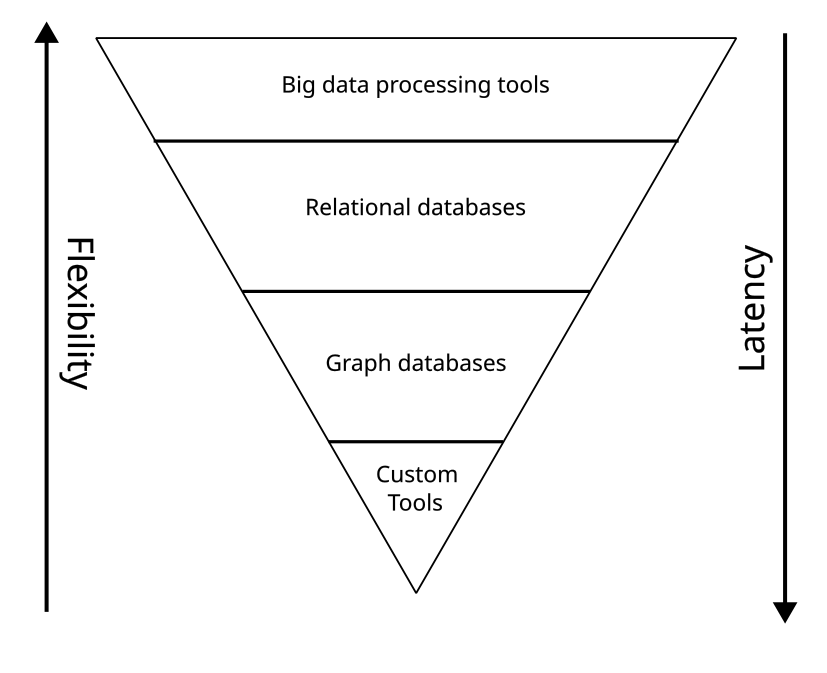
\includegraphics[width=0.5\textwidth]{figures/competitors}
    \caption{Overview of competitors}
    \label{fig:competitorsOverview}
\end{figure}

\smallskip
Within the landscape we have described above, we will compare our tool with
Neo4j, which is a graph database, and Apache Flink, which is a big data
processing framework. Although it is also possible to compare our tool with
relational databases, their wide variety makes it difficult to make a definitive
statement about all relational databases based on a comparison with one of them.
Furthermore, if a relational database does not separate its storage and compute,
then the findings of Section \ref{sec:neo4jCmp} would apply to that database.
However, if it does separate its storage and compute, then it may provide the
same benefits but it will still have worse performance because of less efficient
joins\cite{kotiranta2022performance}.

\subsection{Neo4j}\label{sec:neo4jCmp}
Neo4j\cite{neo4j} was one of the first native graph database and is widely
considered to be the most popular and widely used graph database. The community
version of Neo4j is free to use and its source code is hosted on github.
However, there are a few features that we use for this evaluation that are only
available in the paid enterprise edition.

\subsubsection{Standard Deployment}
% Grammar check from here.
In this section we evaluate the performance of a standard Neo4j deployment.
In this deployment, a single node contains all the relevant information to
answer any query related to the graph. There are various methods of performing
traversal in Neo4j. If we want the highest degree of control over graph
accesses, we can use the `Low-level API'. Then, we have the `Traversals API' which
enables us to provide specifications for a traversal instead of implementing the
core traversal algorithm. Lastly, we can also get the desired results by writing
a cypher query to get the desired results. All three APIs provide the same final
result but use different underlying mechanisms to get those results.

\smallskip
Figure \ref{fig:neoStandardCmp} compares the performance of the three APIs
mentioned in the previous paragraph with S3 One-Zone. The queries shown in this
figure were run on the SF-1 dataset. It is quite apparent from this figure that
regardless of the API used, Neo4j performs an order of magnitude better than
AWS S3. This result is expected because, unlike our service, Neo4j does not have 
to make any network calls. However, this approach of keeping the entire graph on
a single node can not scale indefinitely. Therefore, Neo4j provides composite
databases which enable us to partition the database across various Neo4j nodes. 
\begin{figure}[ht]
    \centering
    \includegraphics[width=0.5\textwidth]{figures/charts/neo4j_bfs_query}
    \caption{Neo4j: Standard Deployment Comparison}
    \label{fig:neoStandardCmp}
\end{figure}

\smallskip
Before talking about composite databases, we note that Neo4j also provides a
graph data science library(GDS) which can also be used to perform traversals.
This library has in-built implementations for common traversal algorithms and a
Pregel API. However, in order to use this library, we need to create an
in-memory projection of the sub-graph that we want to query. Furthermore, this
projection can not be mutated like a normal graph in Neo4j. During our
experiments, we found this library to be less performant than the native Neo4j
APIs for our use-case.

\subsubsection{Composite Databases}
Composite databases in Neo4j consist of multiple standard databases which can be
queried, with special syntax, while using a single database. The main idea
behind using composite databases is that one could partition the graph into
subgraphs such that most of the queries can be served using a single subgraph or
by using a scatter-gather approach. If the graph can indeed be partitioned in
such a way that most of the queries either use a single subgraph or can be
formulated as scatter-gather queries, then the overall performance should be
comparable to what we saw in the previous section. This approach may work well
for some graphs, however, we explore the performance characteristics of this
approach when we are not able to form such isolated partitions of our graph.

\smallskip
When the partitioning of a graph, as described in the previous paragraph is not
possible, then, in the worst case, every step of the traversal might need to be
performed on a different shard. For example, if we want to find the work
locations of a person's friends, and the Person entity is present in a separate
database from the Organization entity, then we would have to wait for results
from one database before we can issue a query to the other database. In this
case, we notice that the query performance degrades severly.

\smallskip
Figure \ref{fig:neoFabricCmp} shows the performance of composite databases where
every alternate hop is performed on a separate database similar to the example
we provided in the previous paragraph. In this figure, we see that the query
performance becomes similar to AWS S3 general and is worse than AWS S3 One-Zone.
\begin{figure}[ht]
    \centering
    \includegraphics[width=0.5\textwidth]{figures/charts/fabric_bfs_cmp}
    \caption{Neo4j: Composite Deployment}
    \label{fig:neoFabricCmp}
\end{figure}

\smallskip
As mentioned before, it may be possible to avoid this type of suboptimal
partitioning for some databases. However, for the general case where we do not
know the eventual size of various entities of a graph and the queries that 
may be performed in the future, it may not be avoidable. Furthermore, this
approach has the following additional drawbacks:
\begin{enumerate}
    \item \textbf{Distribution transparency}: is one of the primary desireable
        characteristic of any distributed system. This states that the user of a
        system should not be aware of how the data and processing is distributed
        within a distributed system. Neo4j's composite databases violate this
        principle because the onus of partitioning the data falls on the user of
        the system.
    \item \textbf{Special Query language}: To the best of our knowledge, we can
        not use the traversal or low-level API with composite databases.
        Furthermore, we need to specify the database that needs to be used for
        each subquery which requires a rewrite of the standard Cypher queries.
        This may become a bigger problem for users who use object relational
        mappers (ORMs), since most ORMs generate standard cypher queries which
        do not work with composite databases.
    \item \textbf{Shadow nodes}: If two entities, which are in different
        databases, have a connection, then that connection requires a shadow
        node. A shadow node is basically a placeholder for a node that is not
        present in the current database but in a remote database. These shadow
        nodes require additional maintainance overhead.
\end{enumerate}

\bigskip
In conclusion, although Neo4j provides great performance for databases that can
be stored on a single machine, this performance may degrade for larger
databases. This is true for graphs that can not be partitioned into independent
graphs such that, either the queries can be answered using a scatter-gather
approach, or the queries can be answered from a single partition. If this
property does not hold, then the query performance can degrade by an order of
magnitude or more. There are other graph databases, like
tigergraph\cite{tigergraph}, which claim to have
distribution transparency for large graphs. However, these claims are difficult
to validate independently since, unlike Neo4j, they do not have the option for
self-hosting.

\subsection{Apache Flink}\label{sec:flinkCmp}

